\section{Latar Belakang}

\begin{frame}{Latar Belakang}
    \begin{columns}
        \begin{column}{0.6\textwidth}
            \begin{itemize}
                \item Teknologi \textit{Automatic Speech Recognition} (ASR) saat ini masih bias pada bahasa bermodal besar (\textit{high-resource}).
                \item \textbf{Bahasa Minangkabau:}
                \begin{itemize}
                    \item Cenderung berada di level \textit{extremely low-resource} (1,3 jam data latih terbuka).
                    \item Minim standarisasi tulisan ortografis untuk format audio ke teks.
                \end{itemize}
                \item Model generik seperti Whisper \textit{zero-shot} menunjukkan error sangat tinggi ketika menghadapi variasi dialek lokal.
            \end{itemize}
        \end{column}
        \begin{column}{0.35\textwidth}
            \centering
            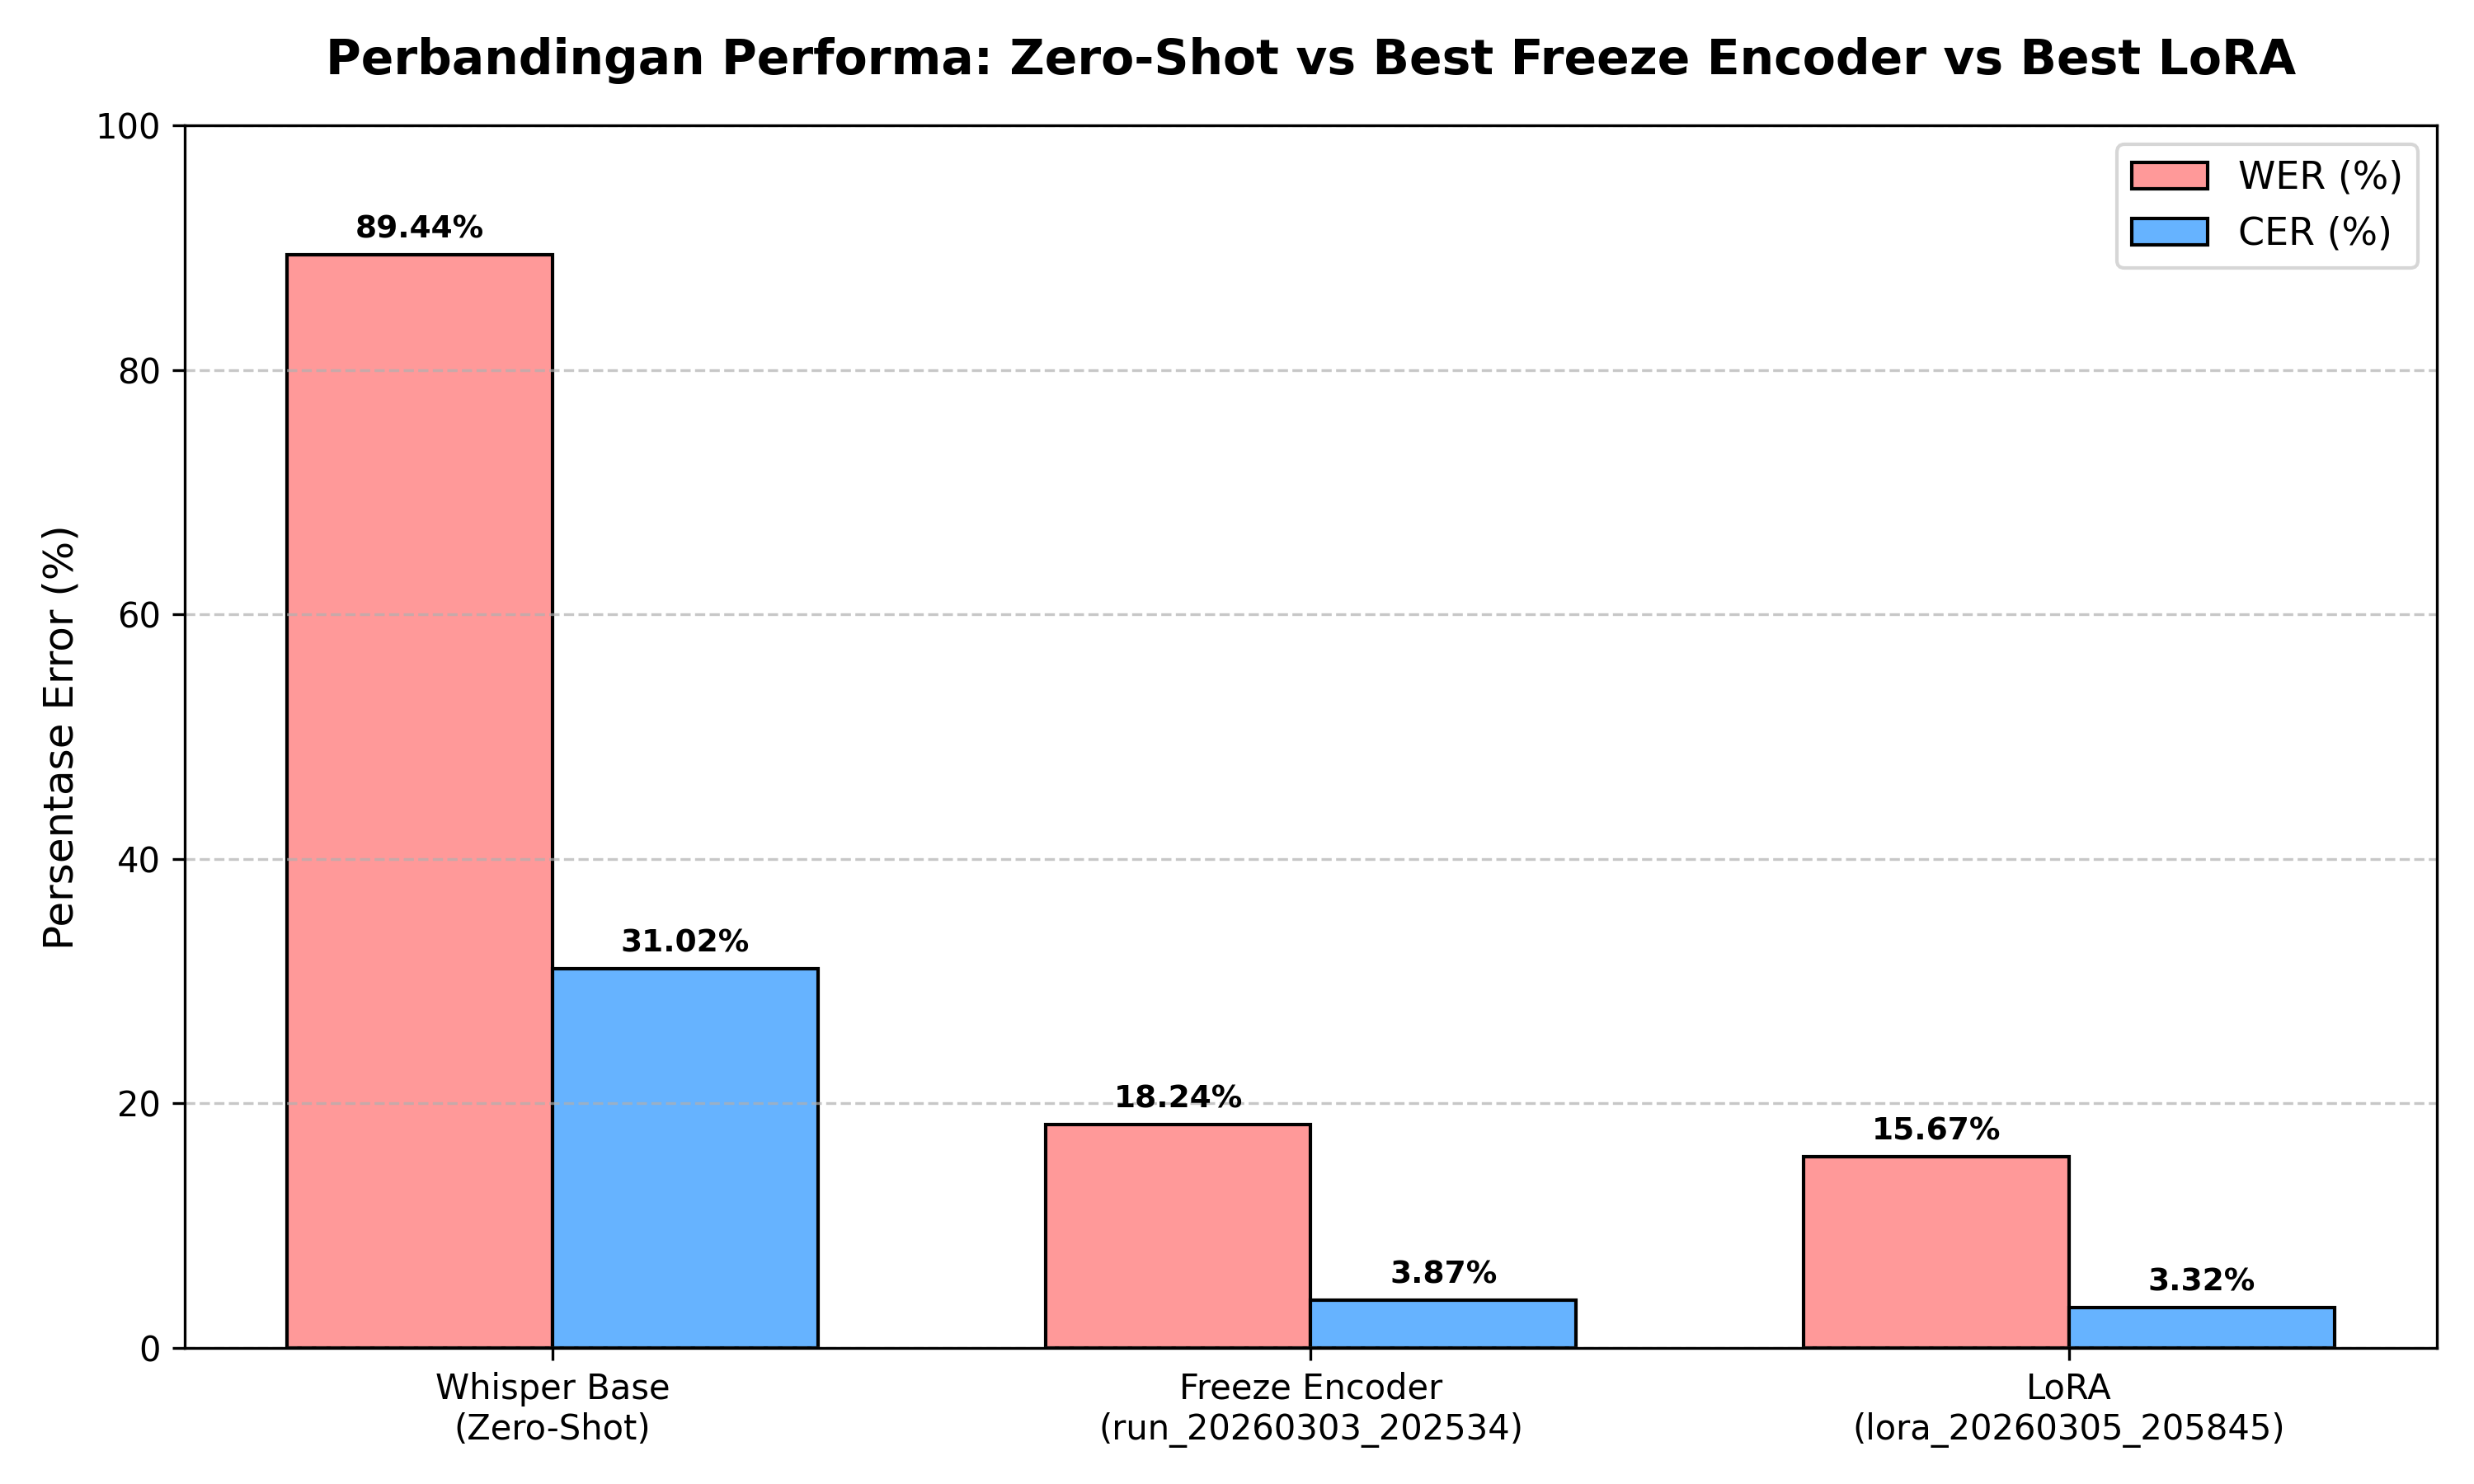
\includegraphics[width=\textwidth]{../figure/zero_shot_comparison.png}
            \vspace{0.2cm}
            \scriptsize Komparasi error \textit{zero-shot} vs run terbaik Freeze Encoder dan LoRA.
        \end{column}
    \end{columns}
\end{frame}

\begin{frame}{Tujuan Penelitian}
    \begin{enumerate}
        \item \textbf{Adaptasi Bahasa Baru:} Melakukan \textit{fine-tuning} model pralatlatih \textit{(pre-trained)} OpenAI Whisper Base ke bahasa Minangkabau.
        \vspace{1em}
        \item \textbf{Komparasi Strategi Efisiensi:} Membandingkan dua strategi efisien: \textit{Freeze Encoder} dan \textit{Low-Rank Adaptation} (LoRA).
        \vspace{1em}
        \item \textbf{Evaluasi Metrik:} Menilai kinerja konversi dari audio menggunakan \textit{Word Error Rate} (WER) dan \textit{Character Error Rate} (CER).
    \end{enumerate}
\end{frame}